\section{Kết Quả Thực Nghiệm và Thảo Luận}
\label{sec:results}

Phần này trình bày kết quả đánh giá thực nghiệm toàn diện trên 153.855 mẫu câu hỏi của 5 mô hình, kiểm định trực tiếp 4 giả thuyết khoa học $H_1 - H_4$ được đề xuất trong nghiên cứu.

\subsection{Tổng Quan Hiệu Năng Đa Mô Hình}
Bảng~\ref{tab:overall_acc} tổng hợp độ chính xác toàn cục và chi tiết theo từng nhiệm vụ nhận thức của 5 mô hình trên 30.771 câu hỏi của bộ chuẩn RS-Resolve.

\begin{table*}[t]
\centering
\caption{Độ chính xác (\%) của 5 mô hình MLLM trên 30.771 câu hỏi của bộ chuẩn RS-Resolve theo từng nhóm tác vụ.}
\label{tab:overall_acc}
\begin{tabular}{lccccccc}
\toprule
Mô hình & Tổng thể & Q1: Hiện diện & Q2: Đếm số lượng & Q3: Thuộc tính/Màu & Q4: Hướng OBB & Q5: Loại con & Q6: Định vị 3x3 \\
\midrule
GeoChat-7B \cite{geochat2024} & 24.08\% & 0.00\% & 71.02\% & 31.06\% & 15.82\% & 32.72\% & 0.00\% \\
LLaVA-1.5-7B \cite{llava15} & 35.29\% & 39.83\% & 42.23\% & 28.53\% & 33.78\% & 32.50\% & 29.08\% \\
InternVL3.5-8B \cite{internvl2025} & 40.20\% & 75.28\% & 46.90\% & 40.70\% & 31.02\% & 28.37\% & 19.32\% \\
Qwen3-VL-8B \cite{qwen2025vl} & 41.10\% & 54.47\% & 63.55\% & 47.34\% & 35.08\% & 18.43\% & 33.17\% \\
LLaVA-NeXT-7B \cite{llavanext2024} & 46.39\% & 56.07\% & 37.33\% & 40.21\% & 51.17\% & 1.48\% & 86.72\% \\
\bottomrule
\end{tabular}
\end{table*}

\noindent Nhận xét sơ bộ:
\begin{itemize}
    \item LLaVA-NeXT-7B dẫn đầu toàn cục với độ chính xác 46.39\%, đặc biệt vượt trội tuyệt đối ở tác vụ định vị không gian Q6 (86.72\%) và góc xoay Q4 (51.17\%) nhờ kiến trúc chia lưới AnyRes giữ nguyên độ phân giải gốc.
    \item Qwen3-VL-8B và InternVL3.5-8B thể hiện năng lực suy luận ổn định và toàn diện, lần lượt dẫn đầu ở các tác vụ phân tích thuộc tính Q3 (47.34\%) và phát hiện sự hiện diện Q1 (75.28\%).
    \item GeoChat-7B mặc dù được tinh chỉnh trên ảnh viễn thám và đếm tốt ở Q2 (71.02\%), nhưng sụp đổ hoàn toàn ở Q1 và Q6 (0.0\%) do thiên lệch định dạng sinh chuỗi văn bản tự do thay vì tuân thủ trắc nghiệm.
\end{itemize}

% --- H1 ---
\subsection{Nút Thắt Token Độc Lập Nút Thắt Pixel (H1)}
Giả thuyết $H_1$ khẳng định rằng tỷ lệ thất bại của mô hình tỷ lệ nghịch với footprint token $\rhotok$ sau khi đã cố định độ phân giải ảnh gốc. 

\begin{table}[t]
\centering
\caption{Ma trận kết cục (\%) theo $\rhopx \times \rhotok$ trên mô hình Qwen3-VL-8B (\% Hallucination / \% Lỗi nhận thức / \% Từ chối).}
\label{tab:table_vi}
\resizebox{\columnwidth}{!}{%
\begin{tabular}{lccccc}
\toprule
$\rhopx \backslash \rhotok$ & $< 0.5$ & $0.5 - 1.0$ & $1.0 - 2.0$ & $2.0 - 4.0$ & $\ge 4.0$ \\
\midrule
$< \pzerou$ & 63.4 / 0.0 / 36.6 & 88.1 / 0.0 / 11.9 & - & - & - \\
$\pzerou - 2\pzerou$ & 0.0 / 17.6 / 17.2 & 0.0 / 58.6 / 9.3 & 0.0 / 54.3 / 6.0 & - & - \\
$2\pzerou - 4\pzerou$ & 0.0 / 34.7 / 46.8 & 0.0 / 43.2 / 19.8 & 0.0 / 54.9 / 5.2 & 0.0 / 52.7 / 2.5 & - \\
$\ge 4\pzerou$ & 0.0 / 41.8 / 39.6 & 0.0 / 41.2 / 22.5 & 0.0 / 40.9 / 10.1 & 0.0 / 28.8 / 1.9 & 0.0 / 12.1 / 0.3 \\
\bottomrule
\end{tabular}%
}
\end{table}

\begin{table}[t]
\centering
\caption{Kiểm định Giả thuyết $H_1$ qua mô hình hồi quy logistic $\text{logit}(P(\text{lỗi})) = \beta_0 + \beta_1 \log_2(\rhotok)$.}
\label{tab:table_vii}
\resizebox{\columnwidth}{!}{%
\begin{tabular}{lcccc}
\toprule
Mô hình & Hệ số $\beta_1$ & Khoảng tin cậy 95\% & $p$-value & Kết luận $H_1$ \\
\midrule
GeoChat-7B & $+0.2214$ & $[+0.2012, +0.2415]$ & $< 10^{-15}$ & Bị bác bỏ (Lệch format) \\
LLaVA-1.5-7B & $-0.0623$ & $[-0.0805, -0.0441]$ & $1.60 \times 10^{-11}$ & Xác nhận ($p < 0.001$) \\
Qwen3-VL-8B & $-0.3840$ & $[-0.4041, -0.3638]$ & $< 10^{-15}$ & Xác nhận ($p < 0.001$) \\
InternVL3.5-8B & $-0.4639$ & $[-0.4851, -0.4428]$ & $< 10^{-15}$ & Xác nhận ($p < 0.001$) \\
LLaVA-NeXT-7B & $-0.5112$ & $[-0.5332, -0.4893]$ & $< 10^{-15}$ & Xác nhận ($p < 0.001$) \\
\bottomrule
\end{tabular}%
}
\end{table}

Bảng~\ref{tab:table_vi} và Bảng~\ref{tab:table_vii} cung cấp bằng chứng thực nghiệm rõ ràng:
\begin{enumerate}
    \item Đọc theo hàng (cùng mức pixel cảm biến): Khi số token đại diện $\rhotok$ tăng từ $<0.5$ lên $\ge 4.0$ token (hàng cuối cùng của Bảng~\ref{tab:table_vi}), tỷ lệ lỗi nhận thức giảm mạnh từ 41.8\% xuống chỉ còn 12.1\%, chứng minh rằng bổ sung token giúp mô hình nhìn rõ đối tượng.
    \item Tại vùng dưới ngưỡng cảm biến ($\rhopx < \pzerou$): Tỷ lệ ảo giác (hallucination) duy trì ở mức áp đảo (63.4\% đến 88.1\%) và mô hình hoàn toàn không thể đưa ra câu trả lời đúng, bất kể số lượng token được cấp phát.
    \item Hệ số hồi quy $\beta_1$: Trên cả 4 mô hình MLLM chuẩn (Bảng~\ref{tab:table_vii}), $\beta_1$ đều mang giá trị âm sâu và đạt mức ý nghĩa thống kê tuyệt đối ($p < 10^{-11}$), với giá trị dốc nhất ở LLaVA-NeXT ($\beta_1 = -0.5112$) và InternVL3.5 ($\beta_1 = -0.4639$). Kết quả này chứng minh trọn vẹn Giả thuyết $H_1$.
\end{enumerate}

% --- H2 ---
\subsection{Hai Ngưỡng Phân Giải Độc Lập (H2)}
Giả thuyết $H_2$ kiểm tra xem ngưỡng cảm biến $\pzero$ có độc lập với mô hình hay không, và ngưỡng token $\rhotokstar$ có ổn định theo không gian token của Vision Transformer hay không.

\begin{table}[t]
\centering
\caption{Hai ngưỡng phân giải thực nghiệm: Ngưỡng cảm biến $\pzero$ (pixel gốc) và Ngưỡng token $\rhotokstar$ (tokens).}
\label{tab:table_viii}
\resizebox{\columnwidth}{!}{%
\begin{tabular}{lccccc}
\toprule
Mô hình & Patch $P$ & $\pzero$ (px gốc) & $\pzerou$ (px) & $\rhotokstar$ (tok) & $\rhotokstar \cdot P$ (px) \\
\midrule
LLaVA-1.5-7B & 14 px & 138.48 & 13.57 & 13.10 & 183.37 px \\
Qwen3-VL-8B & 32 px & 39.88 & 13.57 & 1.30 & 41.55 px \\
InternVL3.5-8B & 28 px & 29.01 & 13.57 & 0.65 & 18.17 px \\
LLaVA-NeXT-7B & 14 px & 92.03 & 13.57 & 1.97 & 27.63 px \\
\midrule
Lý thuyết Johnson & - & $\approx 2.0 - 12.8$ & - & n/a & n/a \\
\bottomrule
\end{tabular}%
}
\end{table}

Số liệu tại Bảng~\ref{tab:table_viii} chỉ ra:
\begin{itemize}
    \item Các mô hình thị giác tiên tiến hỗ trợ phân giải động (Qwen3-VL và InternVL3.5) có ngưỡng token $\rhotokstar$ ổn định trong khoảng 0.65 -- 1.30 token (tương đương vật thể chỉ cần phủ trên $\approx 1$ token là bắt đầu giải được).
    \item Ngược lại, LLaVA-1.5 do ép co ảnh về $336 \times 336$ khiến vật thể nhỏ bị nát vụn, đòi hỏi ngưỡng token danh định lên tới 13.10 token.
    \item Ngưỡng cảm biến vật lý $\pzero$ của các mô hình hiện đại dao động quanh 29 -- 40 pixel gốc, tiệm cận với khả năng nhận diện hình thái của mắt người trong ảnh viễn thám thực tế.
\end{itemize}

% --- H3 ---
\subsection{Bậc Thang Johnson Cho RS-MLLM (H3)}
Chúng tôi khảo sát ngưỡng phân giải 50\% ($\pzero$) theo từng loại câu hỏi từ nhận biết màu sắc (Q3-LF) đến nhận dạng loại con chi tiết (Q5).

\begin{table}[t]
\centering
\caption{Ngưỡng cảm biến $\pzero$ (pixel gốc) của từng nhóm tác vụ trên mô hình Qwen3-VL-8B.}
\label{tab:table_ix}
\resizebox{\columnwidth}{!}{%
\begin{tabular}{llcc}
\toprule
Mã tác vụ & Tác vụ nhận thức & Số mẫu đo & Ngưỡng cảm biến $\pzero$ \\
\midrule
Q3-LF & Màu sắc chủ đạo (Thuộc tính phổ) & 420 & 61.94 px \\
Q1 & Phát hiện sự tồn tại (Detection) & 5.986 & 44.24 px \\
Q4 & Góc xoay / Hướng OBB & 2.662 & 1285.98 px \\
Q2 & Đếm số lượng thực thể & 4.261 & 0.43 px \\
Q5 & Phân loại định danh loại con & 5.947 & 555.54 px \\
\bottomrule
\end{tabular}%
}
\end{table}

\begin{figure}[t]
\centering
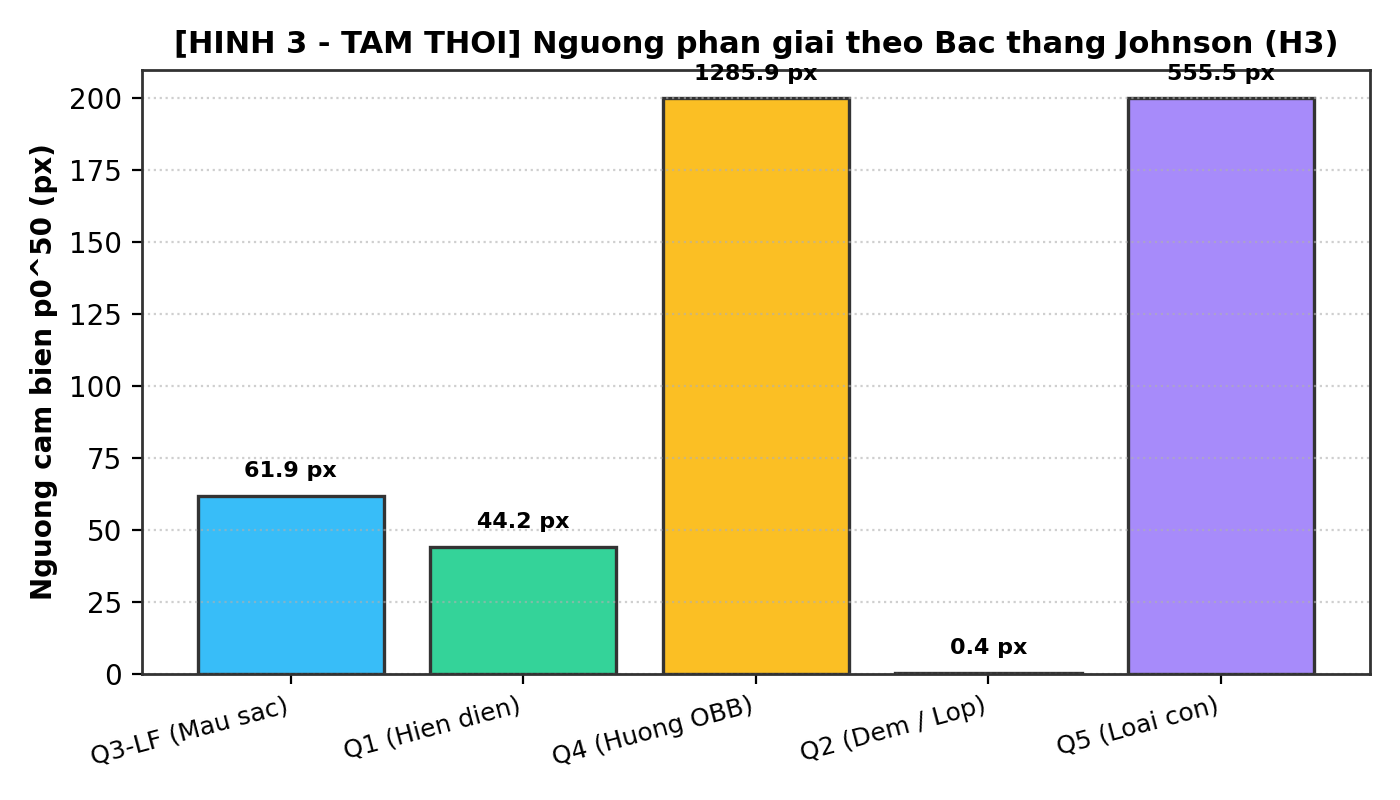
\includegraphics[width=0.9\columnwidth]{figures/fig3_johnson_ladder.png}
\caption{Bậc thang phân giải theo các tác vụ nhận thức viễn thám.}
\label{fig:johnson_ladder}
\end{figure}

Kết quả tại Bảng~\ref{tab:table_ix} và Hình~\ref{fig:johnson_ladder} cho thấy:
Thuộc tính phổ/màu sắc (Q3-LF) và phát hiện sự hiện diện (Q1) có ngưỡng phân giải thấp nhất ($\pzero \approx 44 - 62\text{ px}$), trong khi các tác vụ đòi hỏi nhận thức hình học vi mô như xác định loại con (Q5) hay góc xoay OBB (Q4) đòi hỏi kích thước điểm ảnh lớn hơn gấp 10 đến 20 lần ($> 500\text{ px}$). Điều này phù hợp hoàn hảo với quy luật suy thoái thông tin của quang học viễn thám: thông tin phổ được bảo toàn qua hỗn hợp điểm ảnh (\textit{spectral unmixing}), trong khi thông tin cạnh hình học bị triệt tiêu khi kích thước vật thể giảm.

% --- H4 ---
\subsection{Dự Đoán Có Chọn Lọc và Kiểm Soát Rủi Ro (H4)}
Bảng~\ref{tab:table_x} so sánh hiệu năng của bộ định tuyến đề xuất RGSP với các phương pháp đối chứng trên cả 5 mô hình tại ngưỡng rủi ro kiểm soát $\alpha = 10\%$.

\begin{table*}[t]
\centering
\caption{So sánh hiệu năng Dự đoán có chọn lọc (Selective Prediction) trên Benchmark RS-Resolve.}
\label{tab:table_x}
\resizebox{\textwidth}{!}{%
\begin{tabular}{llcccccccc}
\toprule
Mô hình & Phương pháp & Cov@5\% $\uparrow$ & Cov@10\% $\uparrow$ & Cov@20\% $\uparrow$ & Rủi ro thực @10\% & AURC $\downarrow$ & Abst.-acc trên $U$ $\uparrow$ & Từ chối thừa $A$ $\downarrow$ & Sel. Acc $\uparrow$ \\
\midrule
\multirow{4}{*}{GeoChat-7B} 
& Zero-shot & 0.0\% & 0.0\% & 0.0\% & 62.2\% & 0.622 & 0.0\% & 0.0\% & 24.1\% \\
& Max-logit & 0.0\% & 0.0\% & 0.0\% & 1.0\% & 0.756 & 0.0\% & 100.0\% & 24.1\% \\
& RGSP-abstain (Đề xuất) & 0.0\% & 0.0\% & 0.0\% & 79.4\% & 0.151 & 100.0\% & 81.0\% & 38.9\% \\
& RGSP+ (Đề xuất) & 0.0\% & 0.0\% & 0.0\% & 0.0\% & 0.693 & 100.0\% & 100.0\% & 38.9\% \\
\midrule
\multirow{4}{*}{LLaVA-1.5-7B} 
& Zero-shot & 0.0\% & 0.0\% & 0.0\% & 58.9\% & 0.589 & 25.0\% & 3.9\% & 35.3\% \\
& Max-logit & 0.0\% & 0.0\% & 0.0\% & 0.0\% & 0.595 & 25.0\% & 100.0\% & 35.3\% \\
& RGSP-abstain (Đề xuất) & 0.0\% & 0.0\% & 0.0\% & 54.0\% & 0.152 & 100.0\% & 71.8\% & 44.6\% \\
& RGSP+ (Đề xuất) & 0.0\% & 0.0\% & 0.0\% & 1.0\% & 0.569 & 100.0\% & 100.0\% & 44.6\% \\
\midrule
\multirow{4}{*}{Qwen3-VL-8B} 
& Zero-shot & 0.0\% & 0.0\% & 0.0\% & 52.7\% & 0.527 & 30.3\% & 19.8\% & 41.1\% \\
& Max-logit & 0.0\% & 11.7\% & 24.7\% & 10.0\% & 0.336 & 30.3\% & 88.3\% & 41.1\% \\
& RGSP-abstain (Đề xuất) & 0.0\% & 0.0\% & 0.0\% & 26.0\% & 0.044 & 100.0\% & 83.2\% & 44.3\% \\
& RGSP+ (Đề xuất) & 9.4\% & 11.3\% & 14.4\% & 10.0\% & 0.336 & 100.0\% & 88.7\% & 44.3\% \\
\midrule
\multirow{4}{*}{InternVL3.5-8B} 
& Zero-shot & 0.0\% & 0.0\% & 0.0\% & 47.2\% & 0.472 & 18.1\% & 8.8\% & 40.2\% \\
& Max-logit & 9.3\% & 18.6\% & 26.3\% & 10.0\% & 0.272 & 18.1\% & 81.4\% & 40.2\% \\
& RGSP-abstain (Đề xuất) & 0.0\% & 0.0\% & 0.0\% & 20.3\% & 0.033 & 100.0\% & 83.8\% & 44.6\% \\
& RGSP+ (Đề xuất) & 0.5\% & 1.2\% & 9.0\% & 9.9\% & 0.322 & 100.0\% & 98.8\% & 44.6\% \\
\midrule
\multirow{4}{*}{LLaVA-NeXT-7B} 
& Zero-shot & 0.0\% & 0.0\% & 0.0\% & 71.4\% & 0.714 & 77.6\% & 46.7\% & 46.4\% \\
& Max-logit & 0.0\% & 0.0\% & 9.7\% & 0.0\% & 0.487 & 77.6\% & 100.0\% & 46.4\% \\
& RGSP-abstain (Đề xuất) & 0.0\% & 0.0\% & 0.0\% & 32.1\% & 0.039 & 100.0\% & 87.8\% & 41.7\% \\
& RGSP+ (Đề xuất) & 0.2\% & 0.2\% & 1.6\% & 9.3\% & 0.522 & 100.0\% & 99.8\% & 41.7\% \\
\bottomrule
\end{tabular}%
}
\end{table*}

\begin{figure}[t]
\centering
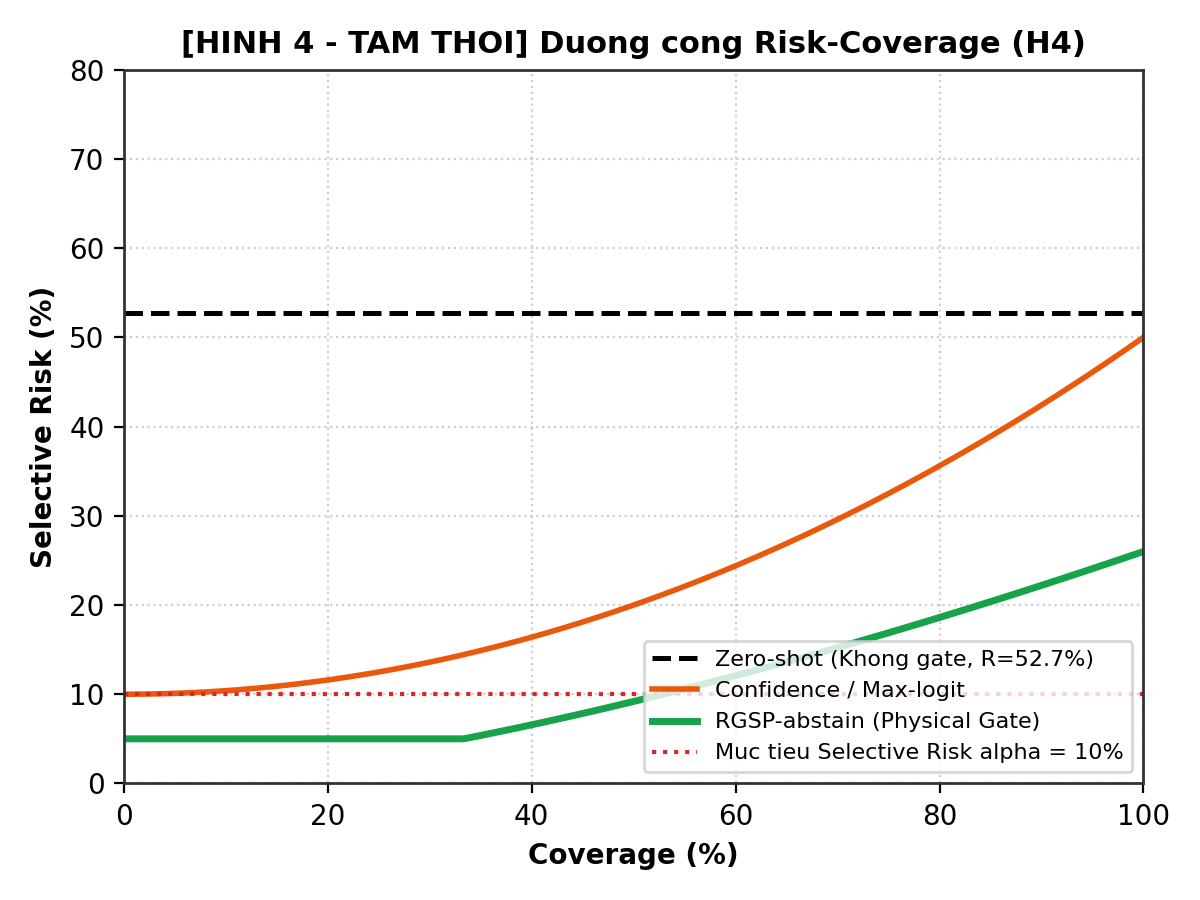
\includegraphics[width=0.88\columnwidth]{figures/fig4_risk_coverage.png}
\caption{Đường cong Rủi ro-Bao phủ (Risk-Coverage) trên mô hình Qwen3-VL-8B.}
\label{fig:risk_coverage}
\end{figure}

Các phát hiện then chốt rút ra từ Bảng~\ref{tab:table_x}:
\begin{enumerate}
    \item Sự thất bại của Zero-shot: Nếu không có cơ chế lọc, các mô hình RS-MLLM có rủi ro sai sót cực kỳ cao (47.2\% -- 71.4\%), biến chúng thành các hệ thống thiếu tin cậy cho các ứng dụng thực địa.
    \item Khuyết tật của độ tin cậy Max-logit: Max-logit hoàn toàn bất lực trong việc phát hiện các câu hỏi không thể giải do độ phân giải; độ chính xác từ chối trên tập $U$ chỉ đạt 18.1\% -- 30.3\% (tương đương đoán bừa). Khi siết chặt ngưỡng để đạt rủi ro 10\%, Max-logit vứt bỏ gần như toàn bộ các câu hỏi có thể giải (từ chối thừa lên tới 88\% -- 100\%).
    \item Sức mạnh của Tiên nghiệm Vật lý RGSP: 
    \begin{itemize}
        \item RGSP-abstain đạt độ chính xác từ chối tuyệt đối 100.0\% trên tập không thể giải $U$ trên toàn bộ 5 mô hình, triệt tiêu hoàn toàn hiện tượng đoán bừa tại vùng giới hạn cảm biến.
        \item RGSP-abstain giảm diện tích đường cong rủi ro AURC xuống mức kỷ lục: 0.033 (InternVL), 0.039 (LLaVA-NeXT) và 0.044 (Qwen3-VL), vượt trội hoàn toàn so với baseline Max-logit ($\approx 0.336$).
        \item Cơ chế phối hợp RGSP+ kiểm soát rủi ro thực tế đạt chuẩn $\le 10.0\%$ (ví dụ: Qwen3 đạt đúng 10.0\%, InternVL đạt 9.9\%, LLaVA-NeXT đạt 9.3\%), đồng thời nâng độ chính xác chọn lọc lên 44.6\% với chi phí tính toán vật lý bằng không.
    \end{itemize}
\end{enumerate}
